\documentclass{beamer}
\usepackage{beamerthemesplit}
\usepackage{wrapfig}
\usetheme{SPbGU}
\usepackage{pdfpages}
\usepackage{amsmath}
\usepackage{cmap}
\usepackage[T2A]{fontenc}
\usepackage[utf8]{inputenc}
\usepackage[english,russian]{babel}
\usepackage{indentfirst}
\usepackage{amsmath}
\usepackage{tikz}
\usepackage{multirow}
\usepackage[noend]{algpseudocode}
\usepackage{algorithm}
\usepackage{algorithmicx}
\usepackage{listings}
\usepackage{pifont}% http://ctan.org/pkg/pifont
\usepackage{xcolor}
\usepackage{mdframed}
\usepackage{multicol}
\usepackage{graphicx}
\usepackage{xspace}
\newcommand{\cmark}{\ding{51}}%
\newcommand{\xmark}{\ding{55}}%

\usepackage{epstopdf}
\usepackage{forest}
\usetikzlibrary{shapes,arrows,positioning}
\usepackage{fancyvrb}
\newtheorem{rutheorem}{Theorem}
\beamertemplatenavigationsymbolsempty
\setbeamertemplate{itemize items}[circle]

\lstdefinelanguage{ocaml}{
%keywords={fresh, let, begin, end, in, match, type, and, fun, function, try, with, when, class,
%object, method, of, rec, %repeat,
%until, while, not, do, done, as, val, inherit,
%new, module, sig, deriving, datatype, struct, if, then, else, open, private, virtual, ostap},
sensitive=true,
basicstyle=\small,
commentstyle=\small\itshape\ttfamily,
keywordstyle=\ttfamily\underbar,
identifierstyle=\ttfamily,
basewidth={0.5em,0.5em},
columns=fixed,
fontadjust=true,
literate={->}{{$\;\;\to\;\;$}}1
         {===}{{$\equiv$}}1
         {&&&}{{$\wedge$}}1
         {|||}{{$\vee$}}1
         {fresh}{{$\exists$}}1,
morecomment=[s]{(*}{*)}
}

\lstset{
basicstyle=\small,
identifierstyle=\ttfamily,
keywordstyle=\bfseries,
commentstyle=\scriptsize\rmfamily,
basewidth={0.5em,0.5em},
fontadjust=true,
%escapechar=~,
language=ocaml,
mathescape=true,
moredelim=[is][\bfseries]{[*}{*]}
}

\definecolor{SadRed}{RGB}{255, 200, 200}
\definecolor{HappyGreen}{RGB}{200, 255, 200}

\newmdenv[backgroundcolor=SadRed, innertopmargin=8,innerbottommargin=1, linecolor=SadRed]{badcode}

\newmdenv[backgroundcolor=MehYellow, innertopmargin=8,innerbottommargin=1, linecolor=MehYellow]{mehcode}

\newmdenv[backgroundcolor=HappyGreen, innertopmargin=8,innerbottommargin=1, linecolor=HappyGreen]{goodcode}

\newcommand{\miniKanren}{\texttt{miniKanren}\xspace}

\title[]{Специализация \miniKanren: почему так сложно}
\institute[]{
Лаборатория языковых инструментов JetBrains
}

\author[Екатерина Вербицкая]{Екатерина Вербицкая}

\date{19 декабря 2020}

\definecolor{orange}{RGB}{179,36,31}

\begin{document}
{

\begin{frame}
      \begin{center}
        {
\includegraphics[width=1.5cm]{pics/jb.png}}
      \end{center}

  \titlepage
\end{frame}
}

\begin{frame}[fragile]
  \frametitle{Реляционное программирование}

 \begin{center}
    Программа --- отношение:
 \end{center}

 \vspace{0.1cm}

  \begin{center}
    \begin{minipage}{3.5cm}
    \begin{lstlisting}[frame=single]
len$^o$ l n =
  (l === [] &&& n === 0)
  ||| (fresh h t m
       ( l === h : t
       &&& n === 1 + m
       &&& len$^o$ t m))
    \end{lstlisting}
    \end{minipage}
\end{center}

\vspace{0.3cm}

\begin{center}
  Выполнение в различных направлениях:
\end{center}

\vspace{-0.1cm}

\begin{columns}
  \begin{column}{0.45\textwidth}
    \begin{center}
      \begin{minipage}{0.45\textwidth}
        \lstinline{len$^o$ [0,1] ? $\rightsquigarrow$ 2}
      \end{minipage}
    \end{center}
  \end{column}
  \begin{column}{0.55\textwidth}
    \begin{center}
      \begin{minipage}{0.55\textwidth}
        \lstinline{len$^o$ ? 2 $\rightsquigarrow$ [$\_.0, \_.1$]}
      \end{minipage}
    \end{center}
  \end{column}
\end{columns}

\end{frame}


\begin{frame}[fragile]
  \frametitle{Реляционные интерпретаторы для синтеза программ}

  \begin{center}
    \begin{minipage}{6.2cm}
    \begin{lstlisting}[frame=single]
eval$^o$ $\subseteq$ Program $\times$ Input $\times$ Output

eval$^o$ p 1 1 &&&  eval$^o$ p 2 1 &&&
eval$^o$ p 3 2 &&&  eval$^o$ p 4 3 &&&
eval$^o$ p 5 5 &&&  eval$^o$ p 6 8
    \end{lstlisting}
    \end{minipage}
    \end{center}
\end{frame}


\begin{frame}[fragile]
  \frametitle{Реализация реляционных
  интерпретаторов}
  \begin{itemize}
    \item Реализовать функциональный интерпретатор
    \item Транслировать функциональный интерпретатор на \miniKanren
    \item Запустить реляционный интерпретатор в обратном направлении
  \end{itemize}

  \vfill

  \begin{itemize}
    \item Транслятор генерирует неэффективный код (в некоторых направлениях)
    \item Специализация помогает избавиться от неэффективности
  \end{itemize}

  \vfill

  \begin{center}
    Lozov, P., Verbitskaia, E. and Boulytchev, D., 2019.

    Relational Interpreters for Search Problems.
\end{center}

\end{frame}

\begin{frame}[fragile]
  \frametitle{Цель и задачи}

\begin{center}
  Разработать методы специализации \miniKanren, которые обеспечивают применимость реляционных интерпретаторов для синтеза
\end{center}

\begin{itemize}
  \item Реализовать консервативную частичную дедукцию для \miniKanren
  \item Поэкспериментировать с суперкомпиляцией для \miniKanren
  \item Реализовать трансляцию реляционных программ в функциональные
  \item Сравнить и выбрать самую адекватную стратегию
\end{itemize}
\end{frame}

\begin{frame}[fragile]
  \frametitle{Специализация для \miniKanren: полное раскрытие}

    \begin{center}
    \begin{minipage}[h]{0.85\textwidth}
      \begin{tikzpicture}[remember picture,overlay,->,node distance=1cm, sibling distance=4cm, scale=0.8, every node/.style={scale=0.8}]
        \tikzstyle{conf}=[rectangle,draw, rounded corners=.8ex,align=center]
        \node[rectangle, draw, anchor=north west, xshift=0.6cm, yshift=-1.7cm] (code) at (current page.north west) {
          \begin{lstlisting}
len$^o$ l n =
  (l === [] &&& n === 0)
  ||| (fresh h t m
        ( l === h : t
        &&& n === 1 + m
        &&& len$^o$ t m))
          \end{lstlisting}
      };
      \node[rectangle, draw, anchor=north east, xshift=-0.6cm, yshift=-1.7cm] (code1) at (current page.north east) {
          \begin{lstlisting}
lenlen$^o$ x y n =
  (x === [] &&& y === [] &&& n === 0)
  ||| (fresh h t h1 t1 m
        ( x === hx : tx
        &&& y === hy : ty
        &&& n === 1 + m
        &&& lenlen$^o$ tx ty m))
          \end{lstlisting}
      };
          \node[conf, right=of code, yshift=-2.5cm, xshift=-0.3cm] (0) {\textit{Unfolding} \\ \lstinline{len$^o$ x n $\wedge$ len$^o$ y n}};
          \node[conf,below left=of 0, xshift=-1.5cm, yshift=-1cm] (10) {\textit{Success} \\ $x \mapsto [],$ \\ $y \mapsto [],$ \\ $n \mapsto 0$};
          \node[conf,right=of 10] (11) {\textit{Fail} \\ $x \mapsto [],$ \\ $y \mapsto (hy:ty)$, \\ $\color{red} n \mapsto 0$ \\ $\color{red} n \mapsto 1 + m$ \\ $\dots$};
          \node[conf,right=of 11] (12) {\textit{Fail} \\ $x \mapsto (hx:tx),$ \\ $y \mapsto [],$ \\  $\color{red} n \mapsto 0$ \\ $\color{red} n \mapsto 1 + m$ \\ $\dots$};
          \node[conf,right=of 12] (13) {\textit{Renaming} \\ $x \mapsto (hx:tx),$ \\ $y \mapsto (hy:ty),$ \\ $n \mapsto 1+m$ \\ \lstinline{len$^o$ tx m $\wedge$ len$^o$ ty m} };

          \draw[>=stealth] (0) -- (10.north east);
          \draw[>=stealth] (0) -- (11.north);
          \draw[>=stealth] (0) -- (12.north);
          \draw[>=stealth] (0) -- (13.north west);

          \draw[>=stealth,dashed] (13) edge [bend right] (0.east);
      \end{tikzpicture}
    \end{minipage}
  \end{center}
\end{frame}

\begin{frame}[fragile]
  \frametitle{Специализация для \miniKanren: раннее расщепление}

    \begin{center}
    \begin{minipage}[h]{0.7\textwidth}
      \begin{tikzpicture}[remember picture,overlay,->,node distance=1cm, sibling distance=4cm, scale=0.8, every node/.style={scale=0.8}, tips=proper]
        \tikzstyle{conf}=[rectangle,draw, rounded corners=.8ex,align=center]
        \node[rectangle, draw, anchor=north west, xshift=0.6cm, yshift=-1.7cm] (code) at (current page.north west) {
          \begin{lstlisting}
len$^o$ l n =
  (l === [] &&& n === 0)
  ||| (fresh h t m
        ( l === h : t
        &&& n === 1 + m
        &&& len$^o$ t m))
          \end{lstlisting}
      };
      \node[rectangle, draw, anchor=north east, xshift=-0.6cm, yshift=-1.7cm] (code1) at (current page.north east) {
        \begin{lstlisting}
lenlen$^o$ x y n =
  len$^o$ x n &&&  len$^o$ y n
        \end{lstlisting}
    };
        \node[conf, right=of code, yshift=-1cm] (0) {\textit{Split} \\ \lstinline{len$^o$ x n $\wedge$ len$^o$ y n}};
        \node[conf, below=of 0, xshift=-3cm] (10) {\textit{Unfolding} \\ \lstinline{len$^o$ x n}};
        \node[conf, below=of 10, xshift=-1.5cm] (20) {\textit{Success} \\ $x \mapsto []$ \\ $n \mapsto 0$};
        \node[conf, below=of 10, xshift=1.5cm] (21) {\textit{Renaming} \\ $x \mapsto (hx:tx)$ \\ $n \mapsto 1+m$ \\ \lstinline{len$^o$ tx m}};
        \node[conf, below=of 0, xshift=3cm] (11) {\textit{Unfolding} \\ \lstinline{len$^o$ y n}};
        \node[conf, below=of 11, xshift=-1.5cm] (22) {\textit{Success} \\ $y \mapsto []$ \\ $n \mapsto 0$};
        \node[conf, below=of 11, xshift=1.5cm] (23) {\textit{Renaming} \\ $y \mapsto (hy:ty)$ \\ $n \mapsto 1+m$ \\ \lstinline{len$^o$ ty m}};


        \draw[>=stealth] (0) -- (10);
        \draw[>=stealth] (0) -- (11);

        \draw[>=stealth] (10) -- (20);
        \draw[>=stealth] (10) -- (21);

        \draw[>=stealth] (11) -- (22);
        \draw[>=stealth] (11) -- (23);

        \draw[>=stealth,dashed] (21) edge [bend right] (10.east);
        \draw[>=stealth,dashed] (23) edge [bend right] (11.east);

        \pause

        \draw[<->, >=stealth, dashed,red] (21.south) [bend right] edge (22.south);
        \draw[<->, >=stealth, dashed,red] (20.south) [bend right] edge (23.south);
      \end{tikzpicture}
    \end{minipage}
  \end{center}
\end{frame}


\begin{frame}[fragile]
  \frametitle{Консервативная частичная дедукция для \miniKanren}
\begin{center}
  Вместо раннего расщепления действуем консервативно:
\end{center}

\begin{itemize}
  \item Временно расщепляем конъюнкцию
  \item Анализируем конъюнкты в изоляции
  \item Если какой-то конъюнкт уменьшает пространство поиска, объединяем конъюнкцию и анализируем ее целиком
  \item Иначе расщепляем конъюнкцию навсегда
\end{itemize}

\vfill

\begin{center}
  Verbitskaia E, Berezun D, Boulytchev D.

  An Empirical Study of Partial Deduction for miniKanren.
\end{center}

\end{frame}

\begin{frame}[fragile]
  \frametitle{Консервативная частичная дедукция: результаты}
  \vspace{-1cm}
  \begin{columns}
    \begin{column}[]{0.4\textwidth}
      \begin{center}
        \scalebox{0.8}{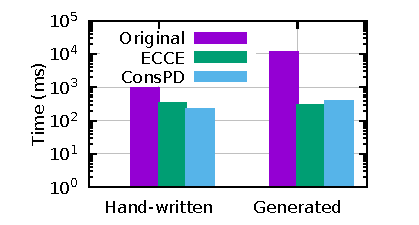
\includegraphics{pics/ltypelog.pdf}}
        \scalebox{0.5}{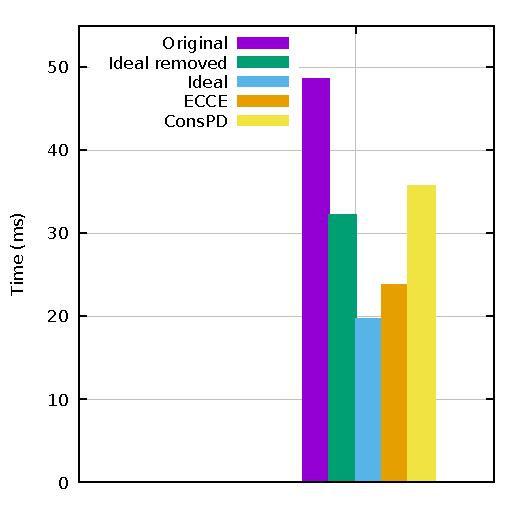
\includegraphics{pics/max.pdf}}
      \end{center}
    \end{column}
    \begin{column}[]{0.6\textwidth}
      \begin{center}
        \scalebox{0.5}{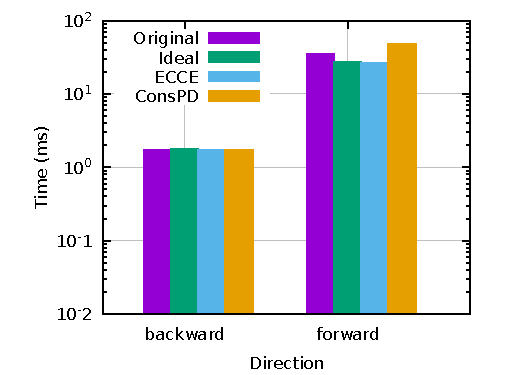
\includegraphics{pics/da700log.pdf}}
        \scalebox{0.5}{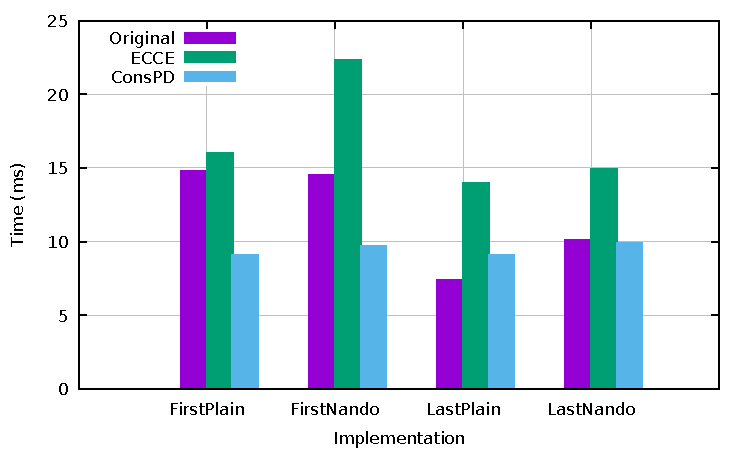
\includegraphics{pics/prop.pdf}}
      \end{center}
    \end{column}
  \end{columns}
\end{frame}

\begin{frame}[fragile]
  \frametitle{Главная причина непредсказуемой производительности}
  \begin{center}
    \miniKanren \textbf{очень} чувствителен к порядку дизъюнктов и конъюнктов
  \end{center}
\end{frame}

\begin{frame}[fragile]
  \frametitle{Влияние порядка дизъюнктов на производительность}
\begin{columns}
  \begin{column}[]{0.5\textwidth}
    \begin{center}
      \begin{minipage}{4.3cm}
      \begin{lstlisting}[frame=single,backgroundcolor = \color{HappyGreen}]
  eval$^o$ p s r =
    (p === Var v    &&&
     lookup$^o$ s v r)
    |||
    (p === Neg x    &&&
     eval$^o$ x s rx &&&
     not$^o$ rx r)
    |||
    (p === Conj x y &&&
     eval$^o$ x s rx &&&
     eval$^o$ y s ry &&&
     and$^o$ rx ry r)
    |||
    (p === Disj x y &&&
     eval$^o$ x s rx &&&
     eval$^o$ y s ry &&&
     or$^o$ rx ry r)
      \end{lstlisting}
      \end{minipage}
  \end{center}
  \end{column}
  \begin{column}[]{0.5\textwidth}
    \begin{center}
      \begin{minipage}{4.3cm}
      \begin{lstlisting}[frame=single,backgroundcolor = \color{SadRed}]
  eval$^o$ p s r =
    (p === Disj x y &&&
     eval$^o$ x s rx &&&
     eval$^o$ y s ry &&&
     or$^o$ rx ry r)
    |||
    (p === Conj x y &&&
     eval$^o$ x s rx &&&
     eval$^o$ y s ry &&&
     and$^o$ rx ry r)
    |||
    (p === Neg x    &&&
     eval$^o$ x s rx &&&
     not$^o$ rx r)
    |||
    (p === Var v    &&&
     lookup$^o$ s v r)
      \end{lstlisting}
      \end{minipage}
  \end{center}

  \end{column}
\end{columns}
\end{frame}

\begin{frame}[fragile]
  \frametitle{Влияние порядка конъюнктов на производительность}
\begin{columns}
  \begin{column}[]{0.5\textwidth}
    \begin{center}
      \begin{minipage}{4cm}
      \begin{lstlisting}[frame=single,backgroundcolor = \color{HappyGreen}]
  len$^o$ l n =
    (l === [] &&& n === 0)
    ||| (fresh h t m
         ( l === h : t
         &&& n === 1 + m
         &&& len$^o$ t m))
      \end{lstlisting}
      \end{minipage}
  \end{center}

  \end{column}
  \begin{column}[]{0.5\textwidth}
    \begin{center}
      \begin{minipage}{4cm}
      \begin{lstlisting}[frame=single,backgroundcolor = \color{SadRed}]
  len$^o$ l n =
    (l === [] &&& n === 0)
    ||| (fresh h t m
         ( l === h : t
         &&& len$^o$ t m
         &&& n === 1 + m))
      \end{lstlisting}
      \end{minipage}
  \end{center}

  \end{column}
\end{columns}
\end{frame}

\begin{frame}[fragile]
  \frametitle{Причина непредсказуемой производительности}
  \begin{center}
    \miniKanren \textbf{очень} чувствителен к порядку дизъюнктов и конъюнктов
  \end{center}

  \vfill

  \begin{itemize}
    \item Производительность измеряется как время, необходимое для получения первых $n$ ответов
    \item При трансляции порядок ответов изменяется
    \item Когда первыми начинают вычисляться более ``сложные'' ответы, на их вычисление требуется больше времени
  \end{itemize}

  \vfill

  \begin{center}
    Но! Специализация уменьшает количество элементарных операций, выполняемых при поиске отдельных ответов
  \end{center}
\end{frame}

\begin{frame}[fragile]
  \frametitle{Что делать?}
  \begin{itemize}
    \item Гарантировать тот же порядок ответов \pause (сложно) \pause
    \item Измерять производительность только на программах, возвращающих конечное множество ответов \pause (бесполезно) \pause
    \item Замерять время, необходимое на каждый ответ \pause (нереалистично) \pause
    \item Подсчитывать количество элементарных операций, выполненных для получения каждого ответа \pause (показательно)
  \end{itemize}
\end{frame}

\begin{frame}[fragile]
  \frametitle{Суперкомпиляция для \miniKanren (Мария Куклина)}
  \begin{center}
    Разработаны и реализованы несколько модификаций суперкомпиляторов для \miniKanren
  \end{center}

  \begin{center}
    Результаты неоднозначные: один и тот же специализатор может как ускорять, так и замедлять программу
  \end{center}
\end{frame}

\begin{frame}[fragile]
  \frametitle{Трансляция из \miniKanren в функциональный язык \ (Ирина Артемьева)}

\begin{itemize}
  \item Учитывается направление вычисления
  \item Производится анализ времени связывания для определения правильного порядка вычислений
\end{itemize}

\begin{itemize}
  \item Функциональные программы работают лучше, чем исходные
  \item Неясно, как определить наиболее оптимальный порядок вызовов рекурсивных функций
  \item Не гарантируется тот же порядок ответов
\end{itemize}

\end{frame}

\begin{frame}[fragile]
  \frametitle{Текущие результаты}
\begin{itemize}
  \item Реализована консервативная частичная дедукция для \miniKanren
  \item Подобрана метрика для сравнения производительности
  \item Реализованы несколько модификаций суперкомпиляции для \miniKanren
  \item Реализован транслятор реляционных программ в функциональные, использующий анализ времени связывания
\end{itemize}
\end{frame}

\begin{frame}[fragile]
  \frametitle{Задачи на будущее}
  \begin{itemize}
    \item Добавить несколько модификаций в консервативную частичную дедукцию
    \item Разработать модель для оценки производительности программ на \miniKanren
    \item Изучить поведение программ после трансляции при выполнении \miniKanren со справедливой конъюнкцией и дизъюнкцией
    \item Доработать транслятор в функциональный язык
  \end{itemize}
\end{frame}

\begin{frame}[fragile]
  \frametitle{Публикации и преподавание}
  \begin{itemize}
    \item Публикации
    \begin{itemize}
      \item Verbitskaia E, Berezun D, Boulytchev D. An Empirical Study of Partial Deduction for miniKanren. (\miniKanren workshop при ICFP)
      \item Артемьева И, Вербицкая Е. Анализ времени связывания для реляционных программ. (SEIM)
      \item Kuklina M, and Verbitskaia E: Supercompilation Strategies of Relational Programs. (TEASE-LP)
      \item Verbitskaia E, Artemeva I and Berezun D: Binding-Time Analysis for miniKanren. (TEASE-LP)
    \end{itemize}
    \item Преподавание
    \begin{itemize}
      \item Лекции и практика по формальным языкам (СПбГУ, ИТМО, ВШЭ, ЛЭТИ)
      \item 2 защищенных магистерских работы
    \end{itemize}
  \end{itemize}


\end{frame}



\end{document}